\section{Proposed methodology}

The proposed two-stream approach will consist of an appearance
stream, representing the static (texture) appearance of each frame,
and a dynamics stream, representing temporal 
variations between frames.
Each stream will consist of a ConvNet whose activation 
statistics will be used to characterize the dynamic texture.
Synthesizing a dynamic texture will be formulated as an optimization 
problem with the objective of matching the activation 
statistics.
My dynamic texture synthesis approach is summarized in Fig.\ \ref{fig:architecture}
and the individual pieces are described in turn in the
following sections.

\begin{figure}[t]
\begin{center}
    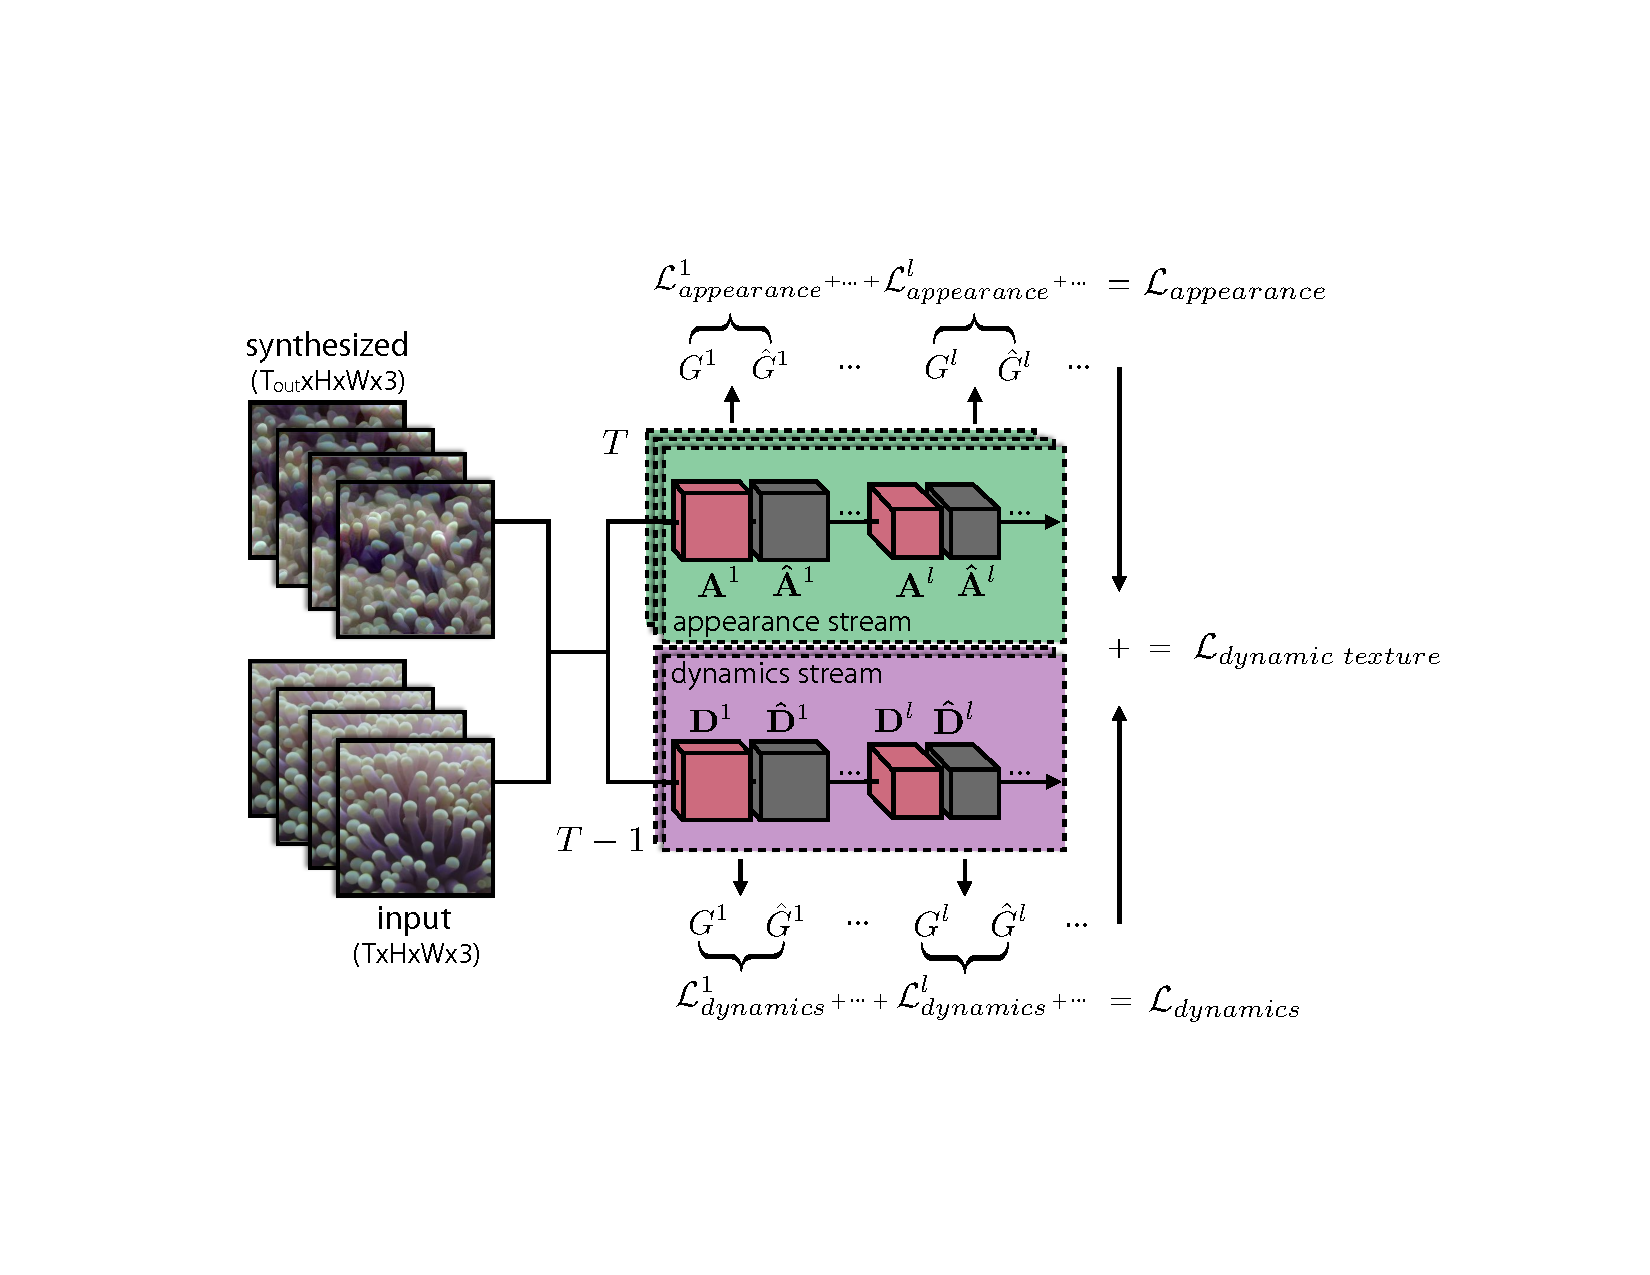
\epsfig{file=overallarchitecture.pdf, width = 0.6\textwidth}
\end{center}
\vspace{-0.45cm}
\caption{Two-stream dynamic texture generation.
Two sets of Gram matrices represent a texture's appearance and 
dynamics.
Matching these statistics will allow for the generation of novel
textures as well as style transfer between textures. Here, $G^l$ and $\hat{G}^l$ are the Gram matrices of activations $A^l$ and $\hat{A}^l$ (or $D^l$ and $\hat{D}^l$) corresponding to the target and synthesized sequence, respectively, computed at layer $l$ of the appearance stream (or dynamics stream) and averaged over time $T$ (or $T-1$). $\mathcal{L}_\text{appearance}^l$ is the appearance loss at layer $l$, computed as the squared Frobenius norm between $G^l$ and $\hat{G}^l$ from the appearance stream. Similarly, $\mathcal{L}_\text{dynamics}^l$ is the dynamics loss at layer $l$ for the dynamics stream. By summing each loss computed at various layers, we arrive at $\mathcal{L}_\text{appearance}$ and $\mathcal{L}_\text{dynamics}$, which, when summed, form the combined dynamic texture loss, $\mathcal{L}_\text{dynamic texture}$, that is to be minimized.}
\label{fig:architecture}
\end{figure}


\subsection{Texture model: Appearance stream}
The appearance stream will follow the spatial texture model
introduced by Gatys et al.\ \cite{gatys2015} which I
briefly review here.
The key idea is that feature correlations in a 
ConvNet trained for 
object recognition  
capture texture appearance.
I will use the same publicly available normalized VGG-19 network \cite{simonyan2014very} used by Gatys et al.\ \cite{gatys2015}.

To capture the appearance of an input dynamic texture, I will first
perform a forward pass with each frame of the image sequence
through the ConvNet and compute the feature activations,
$\mathbf{A}^{lt} \in \mathbb{R}^{N_l\times M_l}$, for various
levels in the network, where $N_l$ and $M_l$ denote
the number of filters and the number of spatial locations of layer
$l$ at time $t$, respectively.
The correlations of the filter responses in a particular layer will be
averaged over the frames and encapsulated by a Gram matrix,
$\mathbf{G}^{l} \in \mathbb{R}^{N_l \times N_l}$, whose
entries are given by
$G_{ij}^l = \frac{1}{T N_l M_l} \sum_{t=1}^T \sum_{k=1}^{M_l} A_{ik}^{lt} A_{jk}^{lt}$,
where $T$ denotes the number of input frames
and $A_{ik}^{lt}$ denotes the activation of feature $i$ at
location $k$ in layer $l$ on the target frame $t$.
The synthesized texture appearance will similarly be represented by a
Gram matrix, $\hat{\mathbf{G}}^{lt} \in \mathbb{R}^{N_l \times N_l}$,
whose activations are given by
$\hat{G}_{ij}^{lt} = \frac{1}{N_l M_l} \sum_{k=1}^{M_l} \hat{A}_{ik}^{lt} \hat{A}_{jk}^{lt}$,
where $\hat{A}_{ik}^{lt}$ denotes the activation of feature $i$ at
location $k$ in layer $l$ on the synthesized frame $t$.
The appearance loss, $\mathcal{L}_\text{appearance}$, is then 
defined as the temporal average of the mean squared error between
the Gram matrix of the input texture and that of the generated
texture computed at each frame:
\begin{equation}
   \mathcal{L}_\text{appearance} = \frac{1}{L_\text{app} T_\text{out}} \sum_{t=1}^{T_\text{out}} \sum_{l} \Vert \mathbf{G}^l - \hat{\mathbf{G}}^{lt} \Vert^2_F\ ,
   \label{eq:apploss}
\end{equation}
where $L_\text{app}$ is the number of layers used to compute Gram
matrices, $T_\text{out}$ is the number of frames being generated in
the output, and $\Vert \cdot \Vert_F$ is the Frobenius norm.
Consistent with previous work \cite{gatys2015}, I will compute Gram matrices on the
following layers: 
\emph{conv1\_1}, \emph{pool1}, \emph{pool2}, \emph{pool3}, and \emph{pool4}.

\subsection{Texture model: Dynamics stream}

There are three primary goals in designing the dynamics stream.
First, the activations of the network must 
represent the temporal variation of the input pattern.
Second, the activations should be largely invariant to the
appearance of the images which should be characterized
by the appearance stream described above.
Finally, the representation must be differentiable to enable 
synthesis.
By analogy to the appearance stream, an obvious choice
is a ConvNet architecture suited for computing
optical flow (\eg, \cite{dosovitskiy2015,ilg2017}) which
is naturally differentiable.
However, with most such models it is unclear how invariant
their layers are to appearance.
Instead, I propose a novel network architecture which is
motivated by the spacetime-oriented energy model
\cite{derpanis2012spacetime,simoncelli1998}.

In motion energy models, the velocity of image content (\ie, motion)
is interpreted as a three-dimensional orientation in the $x$-$y$-$t$
spatiotemporal domain
\cite{adelson1985spatiotemporal,fahle1981,heeger1988,simoncelli1998,watson1983}.
In the frequency domain, the signal energy of a translating
pattern can be shown to lie on a plane through the origin
where the slant of the plane is defined by the velocity of
the pattern.
Thus, motion energy models attempt to identify this 
orientation-plane (and hence the pattern's velocity) via
a set of image filtering operations.
More generally,
the constituent
spacetime orientations for a spectrum of common
visual patterns can serve as a basis for describing the temporal
variation of an image sequence \cite{derpanis2012spacetime}.
This observation suggests that motion energy models may form an
ideal basis for the dynamics stream.

Specifically, I will use the spacetime-oriented energy model
\cite{derpanis2012spacetime,simoncelli1998} to motivate my
network architecture which I briefly review here; 
see \cite{derpanis2012spacetime} for a more in-depth 
description.
Given an input video, 
a bank of oriented 3D
filters, which are sensitive to a range of
spatiotemporal orientations, will be applied.
These filter activations will be rectified (squared) and
pooled over local regions to make the responses robust
to the phase of the input signal, \ie, robust to the
alignment of the filter with the underlying image
structure.
Next, filter activations consistent with the same spacetime
orientation will be summed.
These responses will provide a pixelwise distributed measure
of which orientations (frequency domain planes) are
present in the input.
However, these responses will be confounded by local image
contrast that will make
it difficult to determine
whether a high response is indicative of the presence of
a spacetime orientation or simply due to high image
contrast.
To address this ambiguity, an $\textrm{L}_1$
normalization will be applied across orientation responses which will
result in a representation that is robust to local
appearance variations but highly selective to 
spacetime orientation.

Using this model as my basis, I propose the following 
fully convolutional 
network
\cite{shelhamer2017}.
The ConvNet input will be a pair of temporally consecutive greyscale images.
Each input pair will first be normalized to have zero-mean and unit
variance.
This step will provide a level of invariance to overall
brightness and contrast, \ie, global additive and
multiplicative signal variations.
The first layer will consist of 32 3D spacetime convolution
filters of size $11\times 11 \times 2$
($\text{height} \times \text{width} \times \text{time}$).
Next, a squaring activation function and $5 \times 5$
spatial max-pooling (with a stride of one) will be applied to
make the responses robust to local signal phase.
A $1\times 1$
convolution layer will follow with 64 filters that will combine
energy measurements that are consistent
with the same orientation.
Finally, to remove local contrast dependence, an
$\text{L}_1$ divisive normalization will be applied.

To capture spacetime orientations beyond those capable
with the limited receptive fields used in the initial
layer, I will compute a five-level spatial Gaussian pyramid.
Each pyramid level will be
processed independently
with the same spacetime-oriented energy model and then
bilinearly upsampled to the original resolution and
concatenated.

Prior energy model instantiations (\eg,
\cite{adelson1985spatiotemporal,derpanis2012spacetime,simoncelli1998})
used handcrafted filter weights.
While a similar approach could be followed here, I
opt to learn the weights so that they will be better
tuned to natural imagery.
To train the network weights, I will add additional decoding
layers that take the concatenated distributed
representation and apply a $3\times 3$ convolution
(with 64 filters), ReLU activation, and a $1\times 1$
convolution (with 2 filters) which will yield a two channel
output encoding the optical flow directly.
The proposed architecture is illustrated in
Fig.\ \ref{fig:MSOE}.

\begin{figure}[t]
\begin{center}
    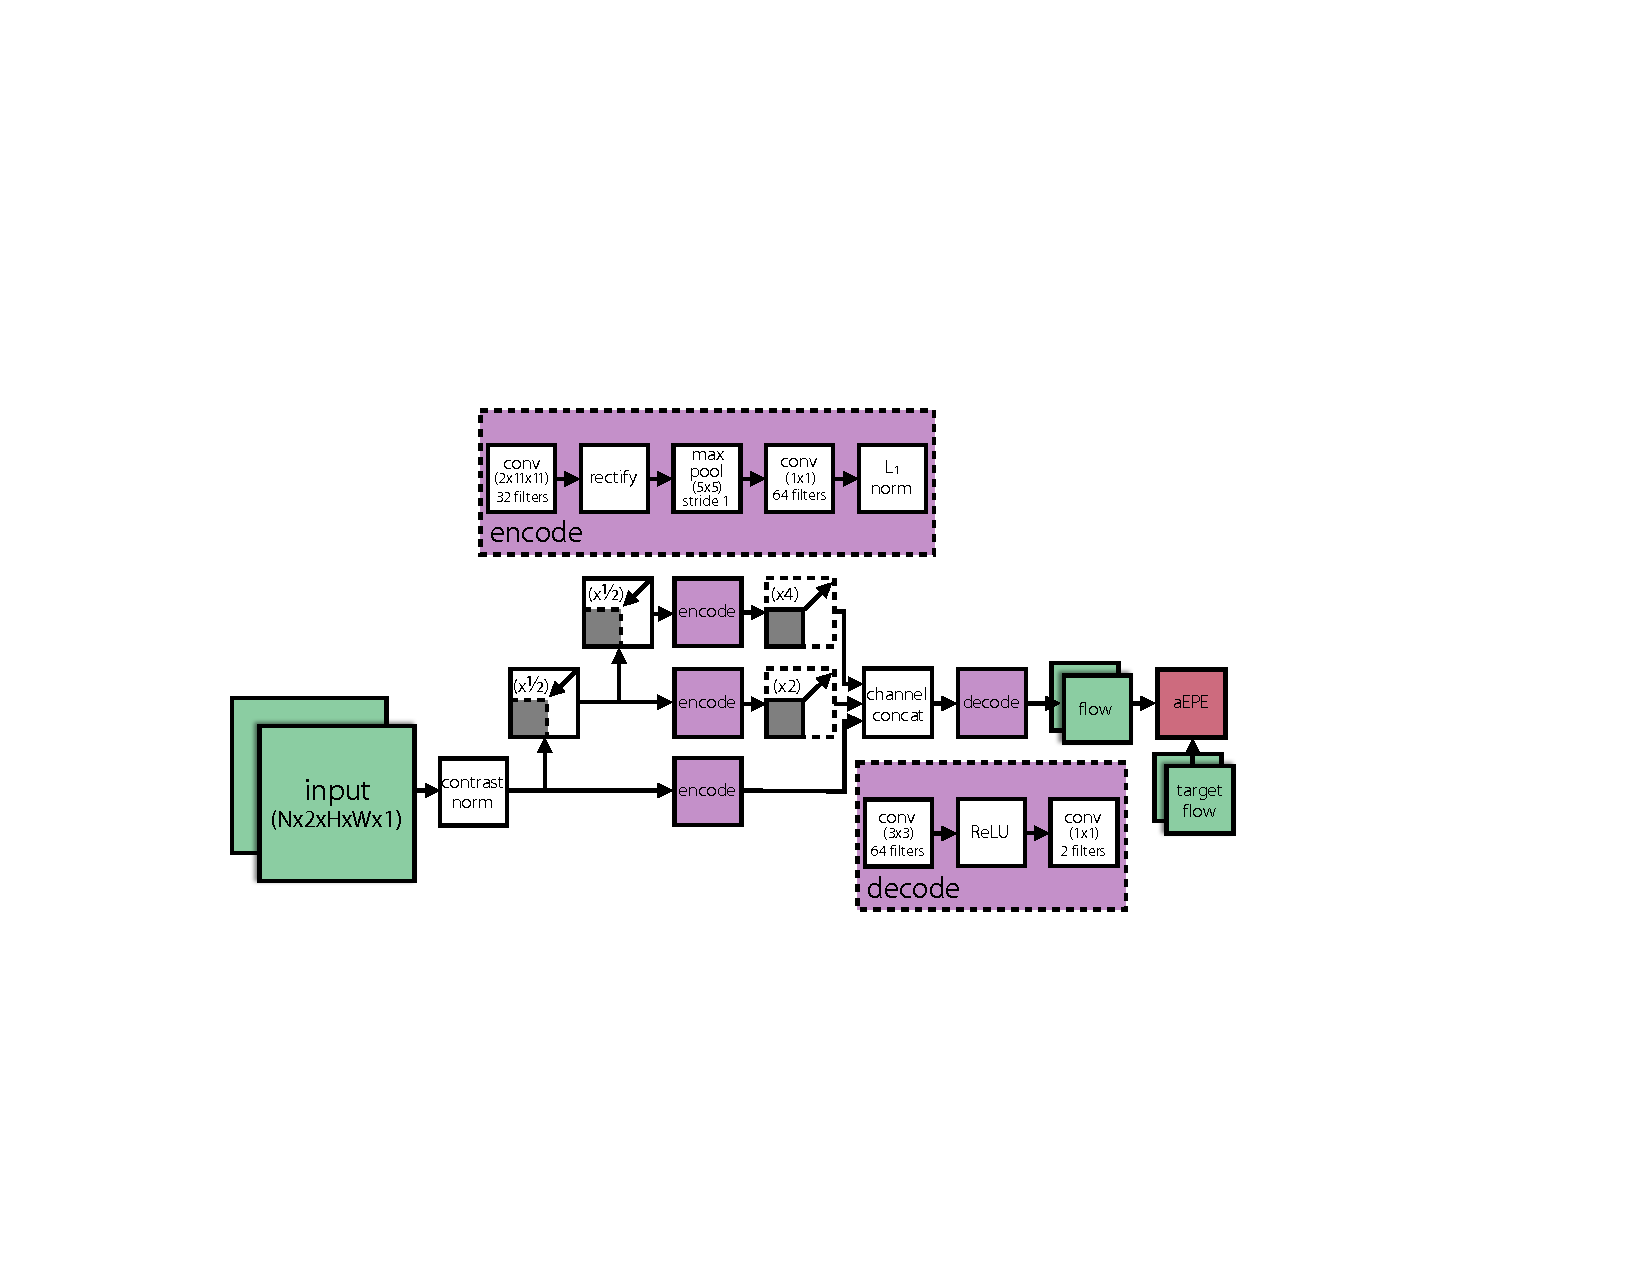
\epsfig{file=MSOEnet.pdf, width = 0.6\textwidth}
\end{center}
\vspace{-0.45cm}
\caption{Dynamics stream ConvNet. The ConvNet is based on a
spacetime-oriented energy model
\cite{derpanis2012spacetime, simoncelli1998} and will be trained
for optical flow prediction.
Three scales are shown for illustration;
in practice five scales will be used.}
\label{fig:MSOE}
\end{figure}

For training, I will use the standard average
endpoint error (aEPE) flow metric (\ie, $\text{L}_2$
norm) between the predicted flow and the ground truth
flow as the loss.
Since no large-scale flow dataset exists that captures
natural imagery with groundtruth flow, I will take an
unlabeled video dataset and apply an existing flow
estimator \cite{revaud2015epicflow} to estimate optical
flow for training,
\cf\ \cite{tran2016}.
For training data, I will use videos from the UCF101
dataset \cite{soomro2012ucf101} with geometric
and photometric data augmentations similar to those used
by FlowNet \cite{dosovitskiy2015}, and optimize the aEPE loss using
Adam \cite{kingma2017}.

Similar to the appearance stream, filter response correlations
in a particular layer of the dynamics
stream will be averaged over the number of image frame
pairs and will be encapsulated by a Gram matrix,
$\mathbf{G}^{l} \in \mathbb{R}^{N_l \times N_l}$,
whose entries are given by
$G_{ij}^l = \frac{1}{(T-1) N_l M_l} \sum_{t=1}^{T-1} \sum_{k=1}^{M_l} D_{ik}^{lt} D_{jk}^{lt}$,
where $D_{ik}^{lt}$ denotes the activation of feature $i$ at
location $k$ in layer $l$ on the target frames $t$ and $t+1$.
The dynamics of the synthesized texture will be represented
by a Gram matrix of filter response correlations 
computed separately for each pair of frames,
$\hat{\mathbf{G}}^{lt} \in \mathbb{R}^{N_l \times N_l}$,
with entries
$\hat{G}_{ij}^{lt} = \frac{1}{N_l M_l} \sum_{k=1}^{M_l} \hat{D}_{ik}^{lt} \hat{D}_{jk}^{lt}$,
where $\hat{D}_{ik}^{lt}$ denotes the activation of feature $i$ at
location $k$ in layer $l$ on the synthesized frames $t$ and $t+1$.
The dynamics loss, $\mathcal{L}_\text{dynamics}$, is defined as
the average of the mean squared error between the Gram matrices
of the input texture
and those of the generated texture:
\begin{equation}
   \mathcal{L}_\text{dynamics} = \frac{1}{L_\text{dyn} (T_\text{out}-1)}\sum_{t=1}^{T_\text{out}-1} \sum_{l}  \Vert \mathbf{G}^l - \hat{\mathbf{G}}^{lt}\Vert^2_F, \label{eq:dynloss}
\end{equation}
where $L_\text{dyn}$ is the number of ConvNet layers being used
in the dynamics stream. Here I propose to use the output of the concatenation layer,
where the multiscale distributed representation of orientations is
stored, as the layer to compute the Gram matrix.

\subsection{Texture generation}\label{sec:texgen}
The overall dynamic texture loss consists of the combination of the appearance loss, Eq.\ (\ref{eq:apploss}),
and the dynamics loss, Eq.\ (\ref{eq:dynloss}):
\begin{equation}
   \mathcal{L}_\text{dynamic texture} = \alpha\mathcal{L}_\text{appearance} + \beta \mathcal{L}_\text{dynamics}, \label{eq:dyntexloss}
\end{equation}
where $\alpha$ and $\beta$ are the weighting factors for the
appearance and dynamics content, respectively.
Dynamic textures will implicitly be defined as the (local) minima 
of this loss.
Textures are generated by optimizing Eq.\ 
(\ref{eq:dyntexloss}) with respect to the spacetime volume,
\ie, the pixels of the video.
Variations in the resulting texture will be found by initializing the
optimization process using IID Gaussian noise.
Consistent with previous work \cite{gatys2015}, I will use
L-BFGS \cite{liu1989} optimization.

\subsection{Dynamics style transfer}
The underlying assumption of my model is that appearance
and dynamics of texture can be factorized.
As such, it should allow for the transfer of the dynamics of
one texture onto the appearance of another.
This has been explored previously for artistic style transfer
\cite{champandard2016,gatys2017} with static imagery.
I will accomplish this with my model by performing the same 
optimization as above, but with the target Gram matrices for 
appearance and dynamics computed from different textures.